\documentclass{../../../lessonplan}
\renewcommand{\cflroot}{../../..}

\begin{document}

\lessonplantitle
    {LKS2-S1}
    {Lower Key Stage 2 Session 1}
    {Recap on using a simple repeat loop}

\preamble
    {
    \item Apply the movement instructions and \keyword{repeat} loops to create a program
    \item Debug the program
    \item Create a challenge for a partner which involves a \keyword{repeat} loop
    }
    {
    \item Levels 19 to 28 in Rapid Router
    \item Resource sheet LKS2-S1-1
    \item Level 21 from Levels Guide
    \item Laptops for group work
    \item Code Wall display space
    \item Interactive Whiteboard (IWB)
    \item LKS2 Assets
    }
    {
    \item Repeat, loop, sequence
    \item Program, algorithm
    \item Move forwards, turn right, turn left
    }

\begin{lessonplan}

\textbf{
Note that you may wish to do the practical element in groups, as each child needs a computer in this session.
You will also need to have shown the children how to log in to the app, using the account details you have created by setting up your class} \textit{[fig S1.1]}.

\fig{fig S1.1}{figS1.1.jpg}{1}

If this is the first time the class has used the app, explain that the turning movements \keyword{turn right} and \keyword{turn left} have a different meaning from the `right' and `left' rotational turn that children may have used with floor robots and Logo-type turtle graphics programming languages.

In the app, \keyword{turn right} means go around the corner in the road from one grid line to the adjacent line on the right \textit{[fig S1.2]}.

\fig{fig S1.2}{figS1.2.jpg}{1}

Ask the children to work out what the \keyword{turn right} and \keyword{turn left} commands do.
You may wish to give the children time to explore levels 1-18 before you start (see Children's previous experience).

Use the level 21 challenge \textit{[fig S1.3]} with a repeated pattern displayed on a large screen or IWB with a sheet between two on the tables.

\fig{fig S1.3}{figS1.3.jpg}{1}

Highlight the blocks of code that are available for them to use (\keyword{move forwards}, \keyword{turn right}, \keyword{turn left}, \keyword{repeat}).
Provide laminated Blockly cards on the tables for children to sequence physically if they need to \textit{[fig S1.4]}.

\fig{fig S1.4}{figS1.4.jpg}{1}


Ask the children, in pairs, to discuss what instructions they will need and write these on their whiteboards.
Discuss their suggestions and ask one pair to key-in their program.
Debug together if needed, to arrive at this \keyword{repeat} loop:

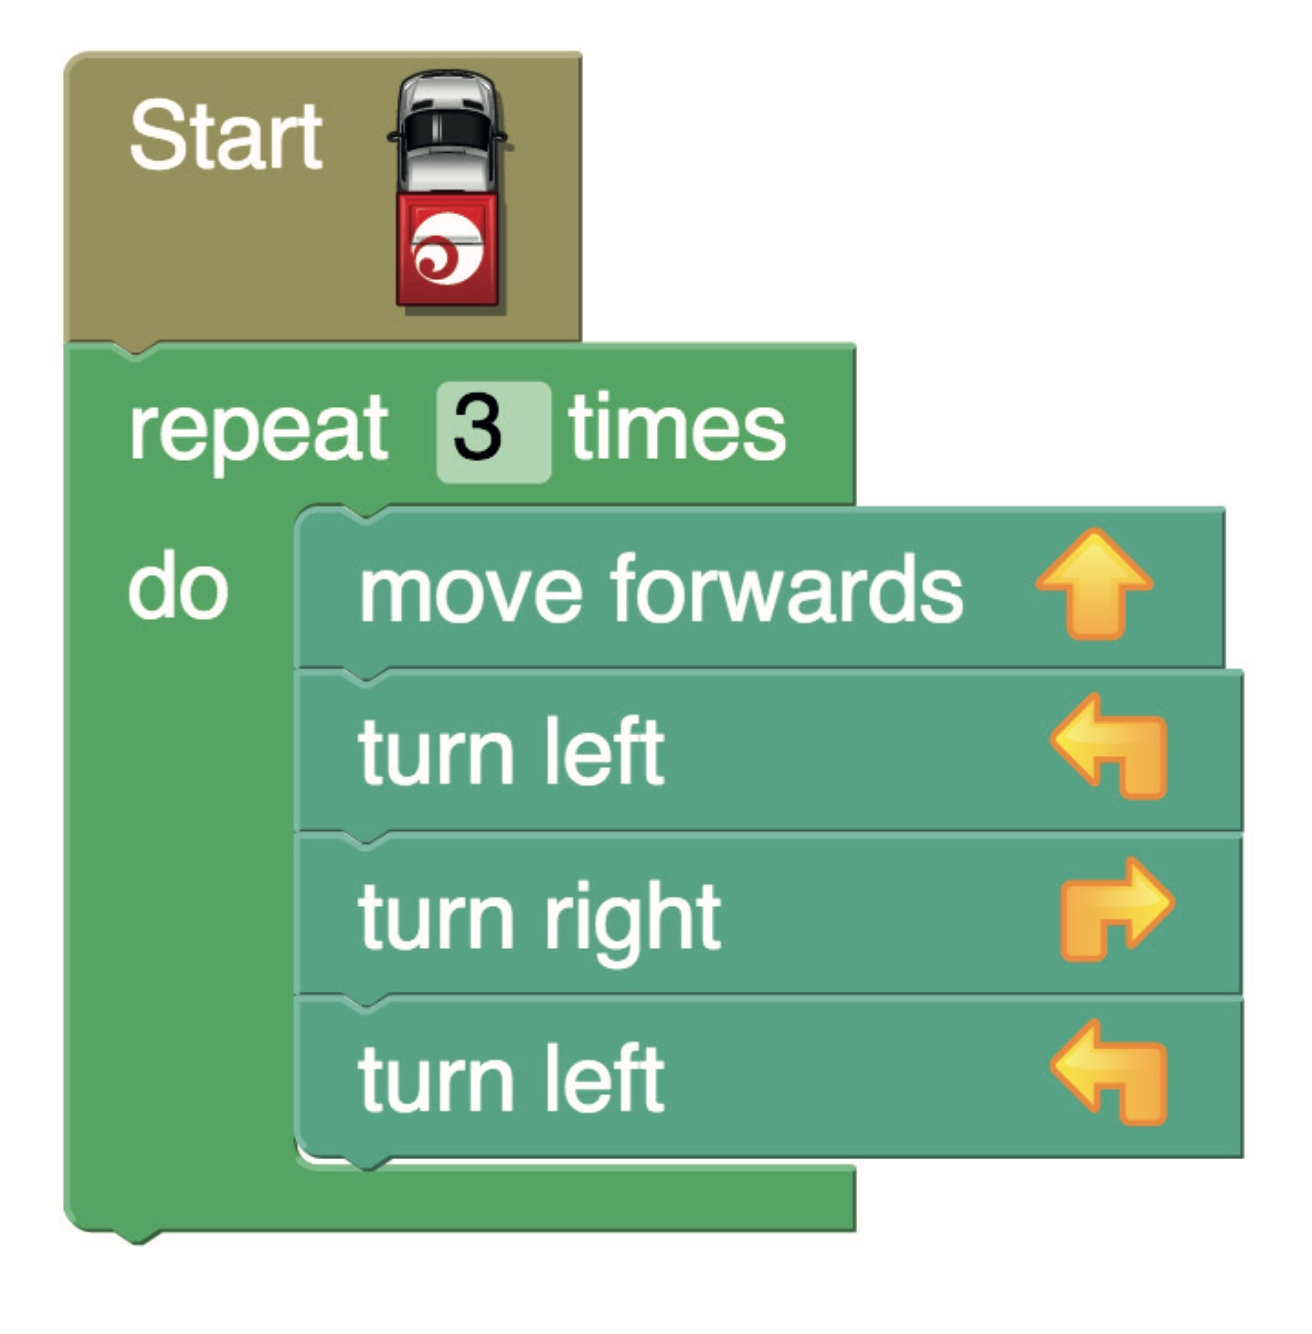
\includegraphics[width=.5\linewidth]{repeat_loop.jpg}


\section*{Practical}

\textbf{1. Practice run}: Children try some of the levels 19-23 individually.

\textbf{2. Challenge your partner}: Show the children how to create their own route.

Explain that they have a short time to create a route for a partner to code, where they will need to use a \keyword{repeat} instruction in their programming.
It could be a simple \keyword{repeat 3 (move forwards)}.

Show level 22 \textit{[fig S1.5]} as an illustration.
Use sheet LKS2-S1-1 to help them plan.
They must then save the route, and test the program themselves to make sure it works.

\fig{fig S1.5}{figS1.5.jpg}{1}

They could take a screen shot and save this to their portfolio/learning record.

\textbf{3. Try out each other's challenge}: Change places and try to code your partner's route (you may prefer to do this in a follow-up session if time is short).

\section*{Extension}

See unplugged activity for gifted and talented pupils in KS1-S8, involving nested \keyword{repeat} loops.

Children can also practice using a simple \keyword{repeat} loop in levels 24 to 28.

\section*{Share and review}

Display two sequences of code next to level 26 \textit{[fig S1.6]} labelled 1 and 2.

\fig{fig S1.6}{figS1.6.jpg}{1}


One sequence is a solution and one is not.

Ask the children to discuss in pairs and write the correct solution on their whiteboards.

\keyquestion{Can you explain how the code works?}

\keyquestion{Is this the shortest possible code sequence?}

This is the correct solution:

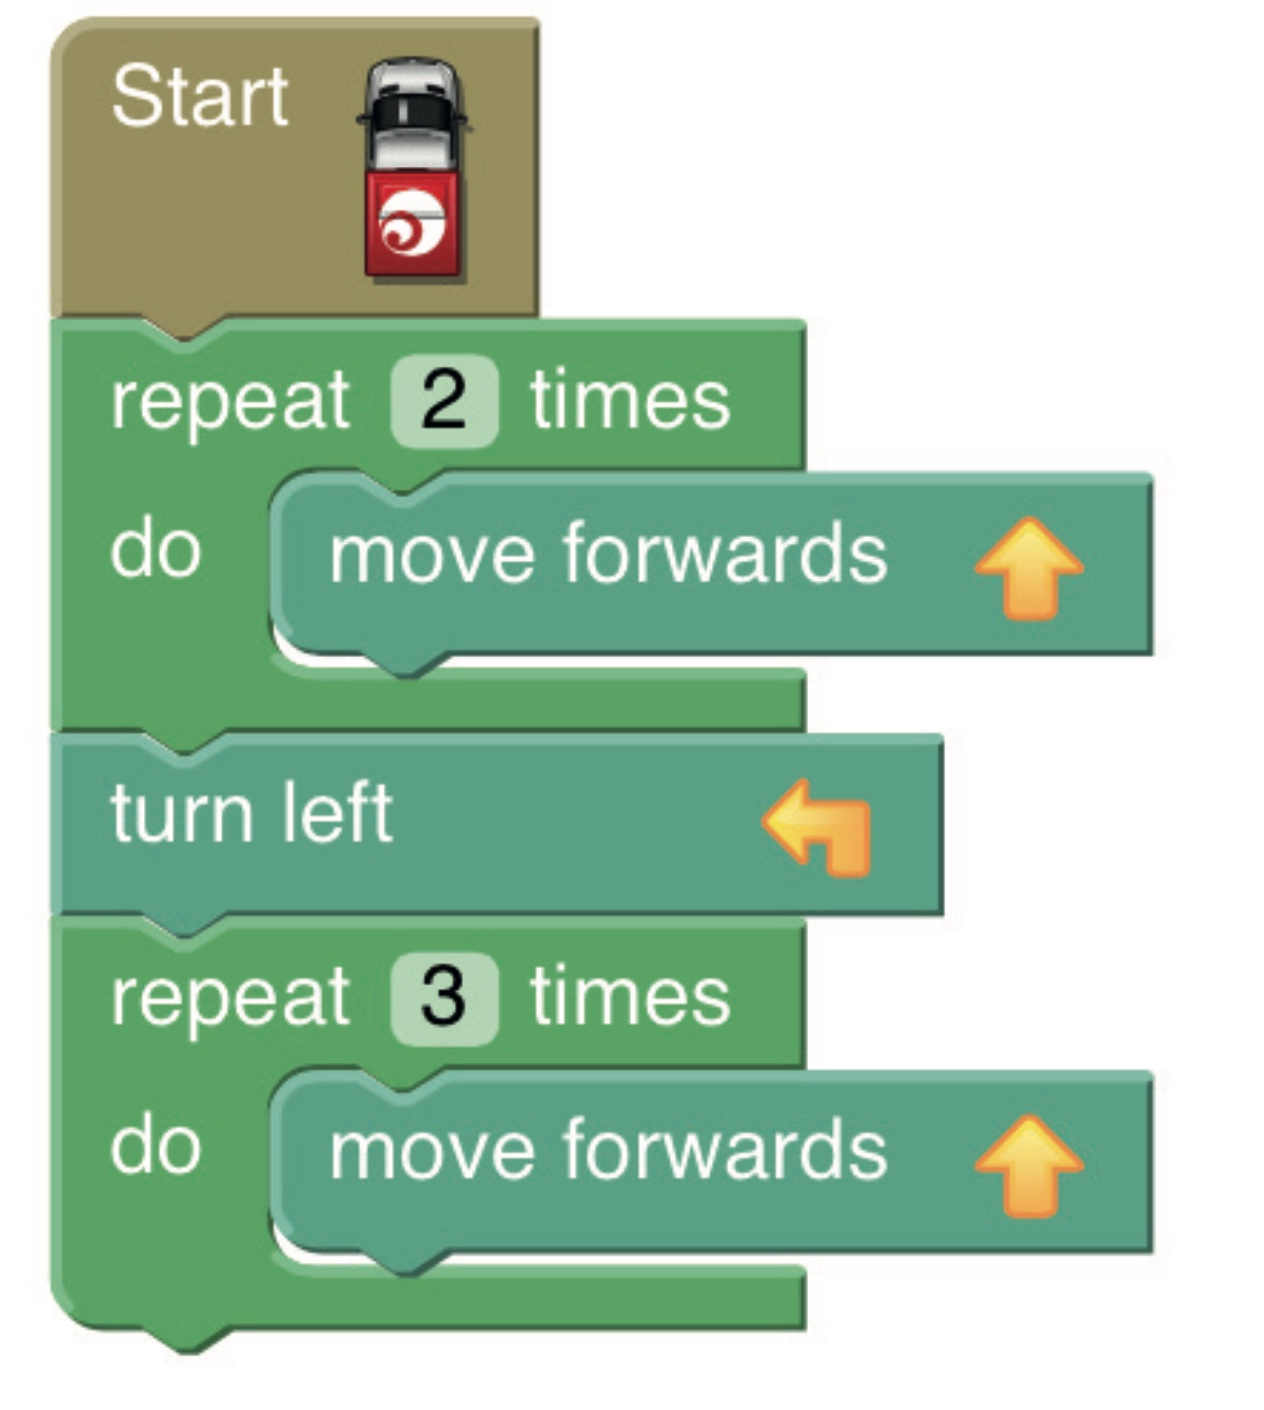
\includegraphics[width=.5\linewidth]{solution.jpg}

\end{lessonplan}

\end{document}
